\subsection{Levinsohn \& Petrin}

\begin{frame}{Levinsohn \& Petrin}
%Last time: 
\bi
	\item{We would like to estimate a firm-level production function}
	\item{Problem: Inputs are endogenous, correlated with a productivity shock $u_{jt}$}
	\item{Solution (Olley \& Pakes): Invert investment function to back out $u_{jt}$}

\begin{align*}
	q_{jt} &= \beta_0 + \beta_kk_{jt} + \beta_\ell\ell_{jt} + u_{jt} + w_{jt}\\
	&= \beta_0 + \beta_kk_{jt} + \beta_\ell\ell_{jt} + h_t(k_{jt}, i_{jt}) + w_{jt}
\end{align*}
	\item{However, the inversion is not feasible for observations with $i_{jt} = 0$. Such observations are dropped.}
	\item{It would be nice to avoid this loss of data $\Longrightarrow$ Levinsohn \& Petrin propose an alternative solution}
	\ei
\end{frame}

\begin{frame}{Levinsohn \& Petrin}
	\textbf{Main idea:} add some freely adjustable input $m_{jt}$ (e.g. materials or energy) and use it as a proxy for productivity shocks $u_{jt}$
	\be
		q_{jt} = \beta_0 + \beta_kk_{jt} + \beta_\ell\ell_{jt} + \beta_mm_{jt} + u_{jt} + w_{jt}
	\ee
	Demand for materials depends on the firm's state variables, $u$ and $k$
	\be
		m_{jt} = m_t(u_{jt}, k_{jt}) \Longrightarrow u_{jt} = m^{-1}_t(m_{jt}, k_{jt}) = h_t(m_{jt}, k_{jt})
	\ee
	Then, as before
	\begin{align*}
			q_{jt} &= \beta_0 + \beta_kk_{jt} + \beta_\ell\ell_{jt} + \beta_mm_{jt} + u_{jt} + w_{jt}\\
			&= \beta_0 + \beta_kk_{jt} + \beta_\ell\ell_{jt} + \beta_mm_{jt} + h_t(m_{jt}, k_{jt}) + w_{jt}\\
			&= \beta_\ell\ell_{jt} + \phi_t(k_{jt}, m_{jt}) + w_{jt}
	\end{align*}
	We assume that $m_t(u,k)$ is a strictly increasing function of $u$.
\end{frame}

\begin{frame}{Identification}
	Proceed in two steps, just as Olley \& Pakes did:
	\begin{enumerate}
		\item{Identify $\beta_\ell$ from
		\be
			q_{jt} = \beta_\ell\ell_{jt} + \phi_t(k_{jt}, m_{jt}) + w_{jt}
		\ee
		where $\phi_t(\cdot)$ is a nonparametric part}
		\item{Identify $\beta_k$ and $\beta_m$ from the second stage equation
		\begin{align*}
			q_{jt} - \beta_\ell\ell_{jt} &= \beta_0 + \beta_kk_{jt} + \beta_mm_{jt} + E[u_{jt}|u_{jt-1}] + \xi_{jt} + w_{jt}\\
			& = \beta_kk_{jt} + \beta_mm_{jt} + \widetilde{g}(\phi_{jt-1} - \beta_kk_{jt-1} - \beta_mm_{jt-1}) + \xi_{jt} + w_{jt}
		\end{align*}
		\bi
			\item{}By definition, $\xi_{jt} = u_{jt} - E[u_{jt}|I_{jt-1}]$ $\Longrightarrow$ $\xi_{jt}$ is orthogonal to what is observed at $t-1$.
			\item{}$w_{jt}$ is orthogonal to anything on the RHS observed at $t$ or prior periods
		\ei
		The combined error is uncorrelated with $k_{jt}$ and $m_{jt-1}$. Approximate $\widetilde{g}(\cdot)$ with a series expansion, then use IV with $k_{jt}$ and $m_{jt-1}$ as instruments.}
	\end{enumerate}
\end{frame}

\begin{frame}{Levinsohn, Petrin}
	\bi
		\item{Main improvement over OP: less data is discarded. Very few firms have zero material inputs, while zero investment may be prevalent.}
		\item{Both require that the proxy variable increases with productivity; this requirement is less intuitive in the case of investment (OP)}
		\item{Both OP and LP methods give reasonable estimates}
	\ei
	However, both have an internal inconsistency that cannot be easily fixed (Ackerberg, Caves, Frazer (2006)).
\end{frame}


\begin{frame}{The ``identifying variation'' question}

\textbf{A side note:} you can hear this question a lot at empirical talks
\begin{block}{}
``What variation in the data identifies $X$ and where does this variation come from?''
\end{block}
The following is a good illustration of why it's important to have an answer.
\end{frame}

\subsection{Ackerberg, Caves, Frazer}
\begin{frame}{Ackerberg, Caves, Frazer}
	First, consider LP
	\bi
		\item{Given $k_{jt}$, labor and materials are perfectly tied to each other via $u_{jt}$
		\begin{align*}
			\ell_{jt} &= \ell_t(u_{jt}, k_{jt})\\
			m_{jt} &= m_t(u_{jt}, k_{jt})\\
			&\Longrightarrow \ell_{jt} = \ell_t(h_t(m_{jt}, k_{jt})) = \psi_t(m_{jt}, k_{jt})
		\end{align*}}
		\item{1st stage equation
		\begin{align*}
			q_{jt} &= \beta_\ell\ell_{jt} + \phi_t(m_{jt}, k_{jt}) + w_{jt}
		\end{align*}}
		\item{\emph{$\beta_\ell$ cannot be identified! Once you fix $m$ and $k$, $\ell$ is fixed, too.}}
	\ei
	The same argument holds for OP -- just replace $m_{jt}$ with $i_{jt}$
\end{frame}

\begin{frame}{Easy ways to fix LP?}
	Intuitively, $\ell_{jt}$ and $m_{jt}$ are tied to each other too rigidly. We would like them to contain some independent variation.
	\bi
		\item{Firm-specific wages and material prices?}
		\item{Dynamic labor?}
		\item{Timing tricks:
		\bi
			\item{$\ell_{jt}$ is chosen before $m_{jt}$}
			\item{$m_{jt}$ is chosen before $\ell_{jt}$}
		\ei}
		\item{Measurement error in $\ell_{jt}$ and $m_{jt}$?}
		\item{Optimization error in $\ell_{jt}$ and $m_{jt}$?}
	\ei
\end{frame}

\begin{frame}{Firm-specific wages and material prices?}
	\bi
		\item{Unobserved: $m_{jt} = m_t(u_{jt}, k_{jt}, p^m_{jt}, p^\ell_{jt}) = \widetilde{m}_{jt}(u_{jt}, k_{jt})$ -- cannot identify the 1st stage equation: the inversion function is firm-specific}
		\item{Observed:
		\begin{align*}
			m_{jt} &= m_t(u_{jt}, k_{jt}, p^m_{jt}, p^\ell_{jt})\\
			\ell_{jt} &= \ell_t(u_{jt}, k_{jt}, p^m_{jt}, p^\ell_{jt})\\
		\end{align*}
		Same problem as before:
		\begin{align*}
			\ell_{jt} &= \psi_t(m_{jt}, k_{jt}, p^m_{jt}, p^\ell_{jt})\\
			q_{jt} &= \beta_\ell\ell_{jt} + \phi_t(m_{jt}, k_{jt}, p^m_{jt}, p^\ell_{jt}) + w_{jt}
		\end{align*}}
	\ei
\end{frame}

\begin{frame}{Dynamic labor?}
	Suppose that labor adjustment has frictions (hiring/firing costs). Then the past labor input becomes a state variable:
	\begin{align*}
		m_{jt} &= m_t(u_{jt}, k_{jt}, \ell_{jt-1})\\
		\ell_{jt} &= \ell_t(u_{jt}, k_{jt}, \ell_{jt-1})\\
	\end{align*}
	Same problem as before:
		\begin{align*}
			\ell_{jt} &= \psi_t(m_{jt}, k_{jt}, \ell_{jt-1})\\
			q_{jt} &= \beta_\ell\ell_{jt} + \phi_t(m_{jt}, k_{jt}, \ell_{jt-1}) + w_{jt}
		\end{align*}	
\end{frame}

\begin{frame}{Timing trick 1: $m_{jt}$ is set before $\ell_{jt}$}
	``Within-period'' timing:
	\begin{description}
		\item[$t-1$:]{End of previous period}
		\item[$t-1/2:$]{Firm observes $u_{jt-1/2}$, chooses $m_{jt}$ based on this information}
		\item[$t$:]{Firm observes $u_{jt}$, chooses $\ell_{jt}$ based on this information}
	\end{description}
	\textbf{Idea:} $u_{jt-1/2}$ contains imperfect information about $u_{jt}$. Additional information that arrives at $t$ creates independent variation in labor.\\\bigskip
	However, in this setting materials are useless as a proxy for $u_{jt}$ for obvious reasons
\end{frame}

\begin{frame}{Timing trick 2: $\ell_{jt}$ is set before $m_{jt}$}
	``Within-period'' timing:
	\begin{description}
		\item[$t-1$:]{End of previous period}
		\item[$t-1/2:$]{Firm observes $u_{jt-1/2}$, chooses $\ell_{jt}$}
		\item[$t$:]{Firm observes $u_{jt}$, chooses $m_{jt}$ based on this information}
	\end{description}
	But then $m_{jt} = m_t(u_{jt}, k_{jt}, \ell_{jt})$, and as before, $\beta_\ell$ is not identified
	\be
			q_{jt} = \beta_\ell\ell_{jt} + \phi_t(m_{jt}, k_{jt}, \ell_{jt}) + w_{jt}
	\ee
\end{frame}

\begin{frame}{A measurement or an optimization error in $m_{jt}$?}
	Let $m_{jt} = m^*_{jt} + \lambda_{jt}$, where $\lambda_{jt}$ may represent
	\bi
		\item{a measurement error: $m^*_{jt}$ is the value actually chosen by the firm}
		\item{an optimization error: $m^*_{jt}$ should have been chosen by the firm, but the firm chose $m_{jt}$}
	\ei
	Then $m_{jt} = m_t(u_{jt}, k_{jt}) + \lambda_{jt}$. The solution for $u_{jt}$ will depend on $\lambda_{jt}$. Proxying $u_{jt}$ with $m_{jt}$ introduces one more unobservable to worry about ($\lambda_{jt}$ is clearly correlated with the observed inputs).
\end{frame}

\begin{frame}{A measurement or an optimization error in $\ell_{jt}$?}
	Let $\ell_{jt} = \ell^*_{jt} + \lambda_{jt}$.
	\bi
		\item{If $\lambda_{jt}$ is a measurement error: this just adds one more error term to the equation ($\beta_\ell\lambda_{jt}$)}
		\item{an optimization error: this may actually work. But do we want to make this assumption? (Remember: there should be no optimization error in $m_{jt}$!)}
	\ei
	\textbf{Verdict:} the situation with LP seems to be hopeless
\end{frame}

\begin{frame}{Olley-Pakes}
	Arguments from the previous slides apply to OP as well. One exception: timing trick with labor chosen first works here
	\begin{description}
		\item[$t-1$:]{End of previous period}
		\item[$t-1/2:$]{Firm observes $u_{jt-1/2}$, chooses $\ell_{jt}$ based on this information}
		\item[$t$:]{Firm observes $u_{jt}$, chooses $i_{jt}$}
	\end{description}
	Then $i_{jt} = i_t(u_{jt}, k_{jt})$. Unlike materials in LP, investment in OP does not depend on labor! (check why)\\\bigskip

	We get what we want: labor and investment have independent variation and
	\be
			q_{jt} = \beta_\ell\ell_{jt} + \phi_t(i_{jt}, k_{jt}) + w_{jt}
	\ee
	One may proceed with the standard OP procedure.\\\bigskip
	Note: By the timing assumption, labor is not fully flexible. Yet it cannot be a dynamic variable like capital -- otherwise $u_{jt} = \phi_t(i_{jt}, k_{jt}, \ell_{jt})$ (check this!). So our modified model is plausible, but shaky.
\end{frame}

\begin{frame}{ACF's suggestion (applicable to OP and LP)}
	\bi
		\item{Keep this timing assumption}
		\item{But don't use 1st stage equation to find $\beta_\ell$. Use it to estimate $\phi_t(i_{jt}, k_{jt}, \ell_{jt})$ only:
		\be
			q_{jt} = \beta_0 + \beta_\ell\ell_{jt} + \beta_kk_{jt} + u_{jt} + w_{jt} = \phi_t(i_{jt}, k_{jt}, \ell_{jt}) + w_{jt}
		\ee
		$\Longrightarrow$ $\widehat{\phi}_{jt} = \widehat\phi_t(i_{jt}, k_{jt}, \ell_{jt})$}
		\item{As before, split $u_{jt}$ into two parts:
		\begin{align*}
			&u_{jt} = E[u_{jt}|I_{jt-1}] + \xi_{jt} = E[u_{jt}|u_{jt-1}] + \xi_{jt} = g(u_{jt-1}) + \xi_{jt}\\
			&\phi_{jt} - \beta_\ell\ell_{jt} - \beta_kk_{jt} = \widetilde{g}(\phi_{jt-1} - \beta_\ell\ell_{jt-1} - \beta_kk_{jt-1}) + \xi_{jt}\\
			&\text{where $\widetilde{g}(x) = g(x - \beta_0) + \beta_0$ --- unknown function}
		\end{align*}
		$\xi_{jt}$ is mean independent of $\ell_{jt-1}$ and $k_{jt}$ (both $\in{}I_{jt-1}$). Use moment conditions $E[\xi_{jt}|\ell_{jt-1}] = E[\xi_{jt}|k_{jt}] = 0$ to identify $\beta_k$, $\beta_\ell$.
		}\\\bigskip
		Now, labor can be a dynamic variable: if labor is dynamic, inverse investment function depends on labor, but that's okay.
	\ei
\end{frame}

\begin{frame}{Empirical exercise}
	\bi
		\item{Chilean plant level data on food products, textiles, wood products and metals}
		\item{Three different proxies for productivity shocks: materials, electricity, fuels. Used separately in LP and ACF estimators}
		\item{Food industry:}
	\ei
	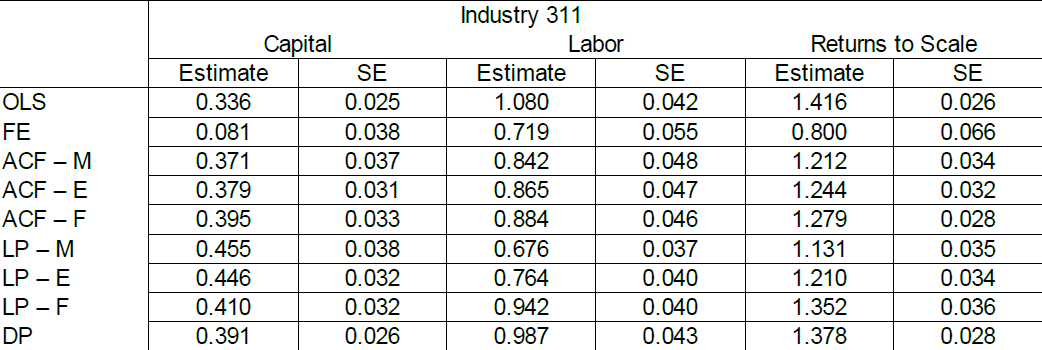
\includegraphics[width=\textwidth]{Figures/acf.png}\\
	Note: LP estimates are unstable. This may be caused by collinearity problems! ACF estimates do not depend so much on the choice of productivity proxy.
\end{frame}